\documentclass[3p, authoryear]{elsarticle} %review=doublespace preprint=single 5p=2 column
%%% Begin My package additions %%%%%%%%%%%%%%%%%%%
\usepackage[hyphens]{url}

  \journal{Journal} % Sets Journal name


\usepackage{lineno} % add

\usepackage{graphicx}
%%%%%%%%%%%%%%%% end my additions to header

\usepackage[T1]{fontenc}
\usepackage{lmodern}
\usepackage{amssymb,amsmath}
\usepackage{ifxetex,ifluatex}
\usepackage{fixltx2e} % provides \textsubscript
% use upquote if available, for straight quotes in verbatim environments
\IfFileExists{upquote.sty}{\usepackage{upquote}}{}
\ifnum 0\ifxetex 1\fi\ifluatex 1\fi=0 % if pdftex
  \usepackage[utf8]{inputenc}
\else % if luatex or xelatex
  \usepackage{fontspec}
  \ifxetex
    \usepackage{xltxtra,xunicode}
  \fi
  \defaultfontfeatures{Mapping=tex-text,Scale=MatchLowercase}
  \newcommand{\euro}{€}
\fi
% use microtype if available
\IfFileExists{microtype.sty}{\usepackage{microtype}}{}
\usepackage{natbib}
\bibliographystyle{apalike}
\usepackage{graphicx}
\ifxetex
  \usepackage[setpagesize=false, % page size defined by xetex
              unicode=false, % unicode breaks when used with xetex
              xetex]{hyperref}
\else
  \usepackage[unicode=true]{hyperref}
\fi
\hypersetup{breaklinks=true,
            bookmarks=true,
            pdfauthor={},
            pdftitle={The Effect of COVID-19 on Utah Traffic Volumes},
            colorlinks=false,
            urlcolor=blue,
            linkcolor=magenta,
            pdfborder={0 0 0}}
\urlstyle{same}  % don't use monospace font for urls

\setcounter{secnumdepth}{5}
% Pandoc toggle for numbering sections (defaults to be off)


% tightlist command for lists without linebreak
\providecommand{\tightlist}{%
  \setlength{\itemsep}{0pt}\setlength{\parskip}{0pt}}

% From pandoc table feature
\usepackage{longtable,booktabs,array}
\usepackage{calc} % for calculating minipage widths
% Correct order of tables after \paragraph or \subparagraph
\usepackage{etoolbox}
\makeatletter
\patchcmd\longtable{\par}{\if@noskipsec\mbox{}\fi\par}{}{}
\makeatother
% Allow footnotes in longtable head/foot
\IfFileExists{footnotehyper.sty}{\usepackage{footnotehyper}}{\usepackage{footnote}}
\makesavenoteenv{longtable}


\usepackage{booktabs}
\usepackage{booktabs}
\usepackage{longtable}
\usepackage{array}
\usepackage{multirow}
\usepackage{wrapfig}
\usepackage{float}
\usepackage{colortbl}
\usepackage{pdflscape}
\usepackage{tabu}
\usepackage{threeparttable}
\usepackage{threeparttablex}
\usepackage[normalem]{ulem}
\usepackage[utf8]{inputenc}
\usepackage{makecell}
\usepackage{xcolor}
\usepackage{booktabs}
\usepackage{longtable}
\usepackage{array}
\usepackage{multirow}
\usepackage{wrapfig}
\usepackage{float}
\usepackage{colortbl}
\usepackage{pdflscape}
\usepackage{tabu}
\usepackage{threeparttable}
\usepackage{threeparttablex}
\usepackage[normalem]{ulem}
\usepackage{makecell}
\usepackage{xcolor}
\usepackage{siunitx}
\newcolumntype{d}{S[input-symbols = ()]}



\begin{document}


\begin{frontmatter}

  \title{The Effect of COVID-19 on Utah Traffic Volumes}
    \author[Brigham Young University]{Matthew Davis\corref{1}}
   \ead{mabosdavis@gmail.com} 
    \author[Brigham Young University]{Gregory Macfarlane\corref{2}}
   \ead{gregmacfarlane@byu.edu} 
      \address[Brigham Young University]{Civil and Environmental Engineering Department, 430 Engineering Building, Provo, Utah 84602}
      \cortext[1]{Corresponding Author}
  
  \begin{abstract}
  We report on the results of an experiment to evaluate the effect of the COVID-19 pandemic on traffic volumes in Orem and Cottonwood Heights, Utah. Linear regression models show that COVID-19 resulted in an 11\% reduction of vehicles per hour on average. Individual signals, month and day of week were controlled for, but signal detector error resulted in a limited number of signals with usable data available for analysis. While only seven signals were used, this methodology in encouraging for future use with more data.
  \end{abstract}
   \begin{keyword} COVID-19, Traffic volumes, ATSPM\end{keyword}
 \end{frontmatter}

\hypertarget{intro}{%
\section{Question}\label{intro}}

Since December 2019, the COVID-19 pandemic has affected life around the world in an unprecedented manner. Mask mandates, social distancing, and stay-at-home orders have changed the way society lives, works, and interacts. With these safety precautions have come less interaction, traveling, and driving on roads and highways. Recent research has confirmed that the COVID-19 pandemic has led to a decrease in traffic volumes across the United States and the world.

Although this is a recent event, the topic has already been researched in many states and countries \citep{Lee2020, Lee2021, Muley2021}, but has not been specifically looked at for Utah and Salt Lake Counties in Utah, USA. These counties also contain signal specific traffic volume detectors, which provide a detailed insight into the variation of the effect of COVID-19 on traffic volumes in different locations. The research question therefore is:

\begin{itemize}
\tightlist
\item
  What was the effect of COVID-19 on traffic volumes in Utah and Salt Lake Counties?
\end{itemize}

\hypertarget{methods}{%
\section{Methods}\label{methods}}

UDOT provided volume data for many signals, but for the purposes of this research, significantly fewer signals were actually analyzed. Data was collected from traffic volume detectors in Provo, Orem, and Cottonwood Heights, Utah and then processed through UDOT's Automated Traffic Signal Performance Measures (ATSPM) system. Data was provided for downtown Provo, Orem State Street, University Avenue, Orem 800 N, and Fort Union Boulevard in Cottonwood Heights for the years 2017-2020, but many of the data were plagued by detector issues. Common issues ranged from shifting of the data up or down considerably and then shifting back after a period of time, missing data, or lack of data in general. Only four signals from Fort Union Blvd and three signals from Orem 800 N were ultimately deemed as complete and consistent enough to be used in the analysis.

Three models were created to evaluate the effect of COVID-19 on volume in the aforementioned corridors. The first was a base model which controlled for variation in volumes at each signal. The second was our base model, but additionally controlling for the effects of COVID-19. The third was the second model, but also controlled for day of the week and month. To divide the Pre COVID-19 time period from the COVID-19 time period, a separation date was chosen. In Utah, on March 12, 2020, Governor Cox announced that gatherings over 100 people should be canceled, as well as many of the universities in the state making the formal announcement that they would transition to online school for the remainder of the semester. These announcements were one of the first events of the pandemic that directly affected the lives of the public in Utah, hence it being chosen as the separation date.

\begin{figure}
\centering
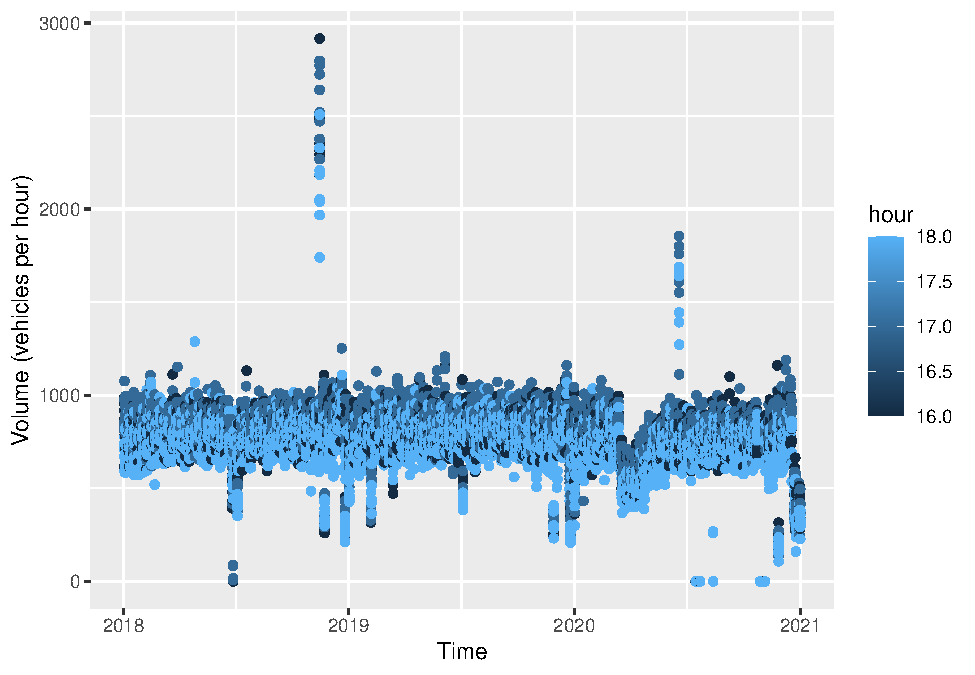
\includegraphics{ATSPM_data_analysis_files/figure-latex/datasummary-1.pdf}
\caption{\label{fig:datasummary}Traffic volumes at Fort Union Blvd and 1300 E in Cottonwood Heights, UT before and during the COVID-19 pandemic.}
\end{figure}

Variation in traffic volumes are dependent on multiple factors such as season, time of day, and day of the week. These three factors were controlled for and were limited to focus the analysis. For days of the week, only Tuesday, Wednesday and Thursday were analyzed. The density of vehicles was greatest during the hours of 7AM to 9AM and 4PM to 6PM, or the ``AM Peak'' and ``PM Peak'' respectively, but only the ``PM Peak'' data were used in the analysis. Other potential factors include weather and road conditions, sporting events and major holidays. Theses were not accounted for in the analysis.

\hypertarget{findings}{%
\section{Findings}\label{findings}}

Table \ref{tab:modeltab} displays the statistical findings of the effects of various variables on traffic volumes. For reference, the ``Intercept'' statistic was used to represent the volume at each signal per phase in vehicles per hour (vph). The ``Base'' model was built such to control for individual signal differences and curiously, signals on the same corridor, denoted by the first number of their signal id, were significantly different in their traffic volumes despite being geographically near each other. Inherently, signals will have different volumes, but the finding that each was significantly different from each other was surprising. The ``COVID'' model showed that after controlling for individual signals, COVID-19 resulted in volumes decreasing by an average of 60 vph. After de-seasonalizing the data in the ``Controls'' model by controlling for month and day of week, the effect of COVID-19 was shown to actually increase additionally to 65 vph. This show that the COVID-19 pandemic resulted in approximately an 11\% reduction in vehicle throughput per signal, on average. The R-squared values increase from 0.515 in the ``Base'' model to 0.524 in the ``Controls'' model, supporting the reduction in error and a closer fit model with the ``Control'' model.

\begin{table}

\caption{\label{tab:modeltab}Traffic Volume Estimates}
\centering
\begin{tabular}[t]{lccc}
\toprule
  & Base & COVID & Controls\\
\midrule
Intercept & \num{597.659}*** & \num{613.964}*** & \num{583.915}***\\
\addlinespace[0.3em]
\multicolumn{4}{l}{\textbf{Signal}}\\
\hspace{1em}4090 & \num{-144.368}*** & \num{-144.014}*** & \num{-143.891}***\\
\hspace{1em}4704 & \num{-256.367}*** & \num{-256.367}*** & \num{-256.367}***\\
\hspace{1em}4705 & \num{-297.147}*** & \num{-297.147}*** & \num{-297.147}***\\
\hspace{1em}6303 & \num{521.797}*** & \num{521.797}*** & \num{521.797}***\\
\hspace{1em}6304 & \num{587.444}*** & \num{587.444}*** & \num{587.444}***\\
\hspace{1em}6307 & \num{361.787}*** & \num{374.462}*** & \num{369.262}***\\
\addlinespace[0.3em]
\multicolumn{4}{l}{\textbf{COVID-19}}\\
\hspace{1em}\textcolor{red}{COVID} & \textcolor{red}{} & \textcolor{red}{\num{-60.470}***} & \textcolor{red}{\num{-64.316}***}\\
\addlinespace[0.3em]
\multicolumn{4}{l}{\textbf{Month}}\\
\hspace{1em}February &  &  & \num{40.496}***\\
\hspace{1em}March &  &  & \num{-4.807}\\
\hspace{1em}April &  &  & \num{-49.007}***\\
\hspace{1em}May &  &  & \num{18.477}***\\
\hspace{1em}June &  &  & \num{68.951}***\\
\hspace{1em}July &  &  & \num{66.158}***\\
\hspace{1em}August &  &  & \num{81.054}***\\
\hspace{1em}September &  &  & \num{67.783}***\\
\hspace{1em}October &  &  & \num{35.628}***\\
\hspace{1em}November &  &  & \num{33.557}***\\
\hspace{1em}December &  &  & \num{18.169}***\\
\addlinespace[0.3em]
\multicolumn{4}{l}{\textbf{Day}}\\
\hspace{1em}Wednesday &  &  & \num{-2.018}\\
\hspace{1em}Thursday &  &  & \num{2.368}\\
\midrule
Num.Obs. & \num{147888} & \num{147888} & \num{147888}\\
R2 & \num{0.515} & \num{0.518} & \num{0.524}\\
F & \num{26192.568} & \num{22729.455} & \num{8127.656}\\
\bottomrule
\multicolumn{4}{l}{\rule{0pt}{1em}Coefficients represent change in traffic volumes per hour.}\\
\multicolumn{4}{l}{\rule{0pt}{1em}t-statistics in parentheses, * p $<$ 0.1, ** p $<$ 0.05, *** p $<$ 0.01}\\
\end{tabular}
\end{table}

Like with any research, there were significant limitations to the data and analyses. Through the data
cleaning process, it became very clear that many of the data provided were not complete or contained
detector errors, leaving most of the data unusable. From 52 signals originally with data, only 7 were used
in this analysis. Even with the most accurate data available, further detector error or unknown errors could
be present. Other factors such as weather, holidays and major events, school openings, weather, and road
conditions were not controlled for.

\hypertarget{acknowledgements}{%
\section{Acknowledgements}\label{acknowledgements}}

We are grateful for the Utah Department of Transportation for supporting this research by providing the traffic volume data. Graphs and plots were created using three open-source R packages \citep{modelsummary, ggplot2, kableExtra}.

\bibliography{book.bib}


\end{document}
